% titlepage-demo.tex
\documentclass{beamer}

% items enclosed in square brackets are optional; explanation below
\title{Flow-Insensitive Points-To Analysis with Term and Set
  Constraints \cite{Foster97flow-insensitivepoints-to}}
\subtitle{Pointer analysis in type theory's clothing!}
\author{Mihir Mehta}
\institute{
  Department of Computer Science\\
  University of Texas, Austin\\
  \texttt{mihir@cs.utexas.edu}
}
\date{20 October, 2014}

\usepackage{amsmath}
\usepackage{graphicx}

\setbeamertemplate{footline}[frame number]
\begin{document}

%--- the titlepage frame -------------------------%
\begin{frame}[plain]
  \titlepage
\end{frame}

\section{Term and set constraints}

\begin{frame}[allowframebreaks]
  \frametitle{Set constraints 101 \cite{DBLP:journals/scp/Aiken99}}
  %% \item Useful for a whole lot of applications
  %%    ranging from register allocation
  %%   to type inference.
  %% \item First formalised \cite{Heintze91adecision} in 1991, solved for good
  %%   \cite{DBLP:conf/focs/CharatonikP94} in 1994.
    \begin{definition}
      Set constraints describe relationships between sets of
      \emph{terms}. They take the form $X \subseteq Y $, where $X$ and
      $Y$ are set expressions, generated by this grammar.
      $ E ::= \alpha | 
      0 | 
      E_1 \cup E_2 | 
      E_1 \cap E_2 | 
      \neg E_1 |
      c(E_1,\dotsc, E_{a(c)})|
      c^{-i}(E_1)$
    \end{definition}
    \begin{definition}
      A system of set constraints is a finite conjunction of
      constraints $ \bigwedge_{i} X_i \subseteq Y_i $.
    \end{definition}
    \begin{definition}
      A solution to a system of set constraints is an assignment
      $ \sigma $ of sets to variables in the system such that all the
      constraints in the system are satisfied when $ \sigma $ is
      extended to set expressions under these rules.
    \end{definition}

    \begin{align*}
      \sigma(0) &= \phi \\
      \sigma(E_1 \cup E_2) &= \sigma (E_1) \cup \sigma (E_2) \\
      \sigma(E_1 \cap E_2) &= \sigma (E_1) \cap \sigma (E_2) \\
      \sigma(\neg E_1) &= H - \sigma (E_1) \\
      \sigma(c(E_1,\dotsc, E_n)) &= \{c(t_1,\dotsc,t_n) | t_i \in \sigma(E_i)\} \\
      \sigma(c^{-i}(E)) &= \{t_i | \exists c(t_1,\dotsc,t_n) \in \sigma(E)\}
    \end{align*}

  \begin{itemize}
    \item H is the Herbrand universe, that is, the set of all terms.
    \item We use $ X = Y $ as a notational convenience to denote the
      pair of constraints $ X \subseteq Y $ and $ Y \subseteq X
      $. In the Hindley-Milner type system, constraints occur only in
      this form, and are solved by unification.
    \item Set constraints, in general, are solved by repeated
      application of re-writing rules, as we shall see.
  \end{itemize}
\end{frame}

\begin{frame}[allowframebreaks]
  \frametitle{This paper}

  \begin{itemize}
  \item Andersen \cite{Andersen94programanalysis} and Steensgard
    \cite{Steensgaard96points-toanalysis} both presented algorithms
    for pointer analysis; this paper formulates both of
    these algorithms as sets of typing rules. 
  \item Typing rules are set constraints and can thus be solved in the
    general framework \cite{F?hndrich97programanalysis} which the
    authors had previously developed.
  \item The resulting implementation (in ML) is compared to a previous,
    more application-specific implementation (in C)
    \cite{Shapiro97fastand}; the former's running time is found to be
    within a small constant factor of the latter.
  \item More concretely, this paper develops typing rules common to
    both algorithms (\boldit{Common}), typing rules specific to each
    algorithm (\boldit{And} and \boldit{Ste}) and shows that the
    type relations/equivalences which arise from
    \boldit{And+Common} and \boldit{Ste+Common} are
    equivalent to the points-to relations in the original algorithms.
  \item Further, the paper shows that the two algorithms are similar
    enough to be represented by a combined set of rules
    (\boldit{Comb}), in which the only difference is in the
    constructor signatures.
  \end{itemize}
\end{frame}

\begin{frame}[allowframebreaks]
  \frametitle {The analysis framework}
  \begin{itemize}
    \item Set of sorts S, including Term and Set.
    \item Each n-ary constructor c has a signature $$ c: \iota_1
      \dotso \iota_n : S $$
      where each $\iota_i$ is $s$ (covariant) or $\overline{s}$
      (contravariant) for some $s \in S$.
    \item Sort Term: set of constructors $\Sigma_{Term}$, 
      set of variables $V_{Term}$. Terms: variables from $V_{Term}$ or
      constructed terms following some constructor's signature:
      $$ c:Term \dotso \underbrace{Term \rightarrow Term}_{arity(c)},
      c \in \Sigma_{Term} $$
    \item Sort Set: set of constuctors $\Sigma_{Set}$, operations
      ${\cup, \cap, 0, 1}$. Set expressions follow some constructor's
      signature: 
      $$ c:Set \dotso \underbrace{Set \rightarrow Set}_{arity(c)},
      c \in \Sigma_{Set} $$
      \begin{figure}
        \centering
        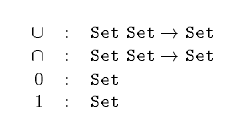
\includegraphics[scale=0.3]{set_operations.png}
      \end{figure}
    \item In general, a sort $s$ has a constraint relation
      $\subseteq_s$ and resolution rules for $\subseteq_s$. Term has
      two, $=_t$ (Hindley-Milner style equality) and $=_c$
      (Steensgard-style conditional equality.).
  \end{itemize}

  \begin{figure}
    \centering
    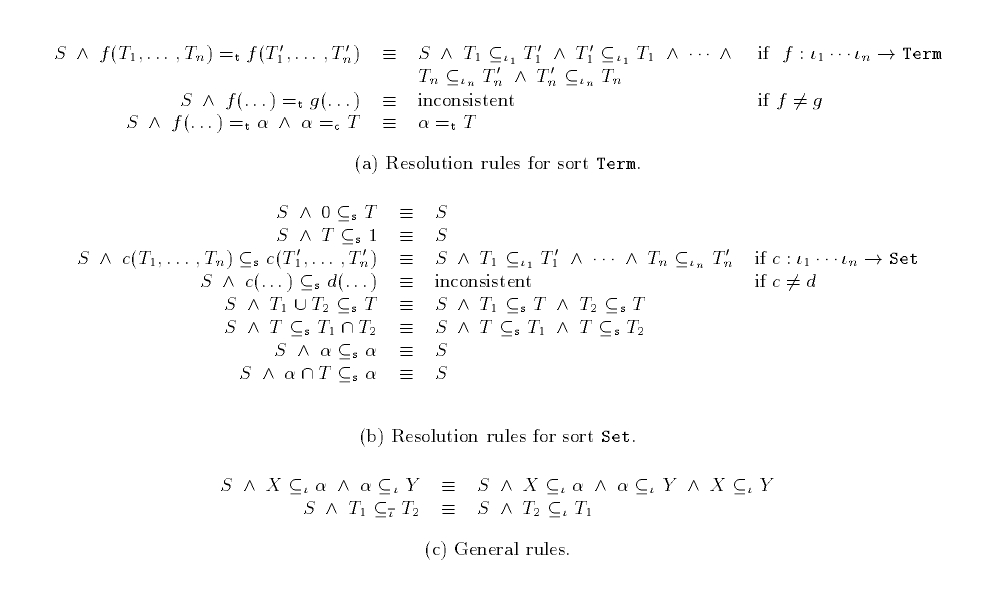
\includegraphics[scale=0.3]{resolution_rules.png}
  \end{figure}

\end{frame}

\begin{frame}[allowframebreaks]
  \frametitle{Andersen-style analysis}
  We analyse this fragment of C. Note that this excludes several
  control-flow constructs such as for loops, while loops and goto
  which are redundant under flow-insensitivity.

  \begin{figure}
    \centering
    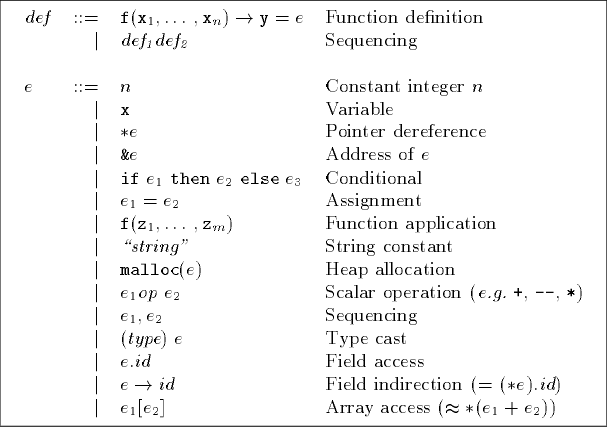
\includegraphics[scale=0.3]{language_syntax.png}
  \end{figure}

  \framebreak

  \begin{itemize}
  \item In this system, types follow this grammar.
    \begin{figure}
      \centering
      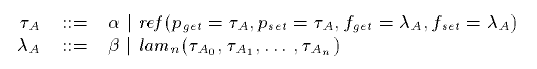
\includegraphics[scale=0.3]{andersen_type_grammar.png}
    \end{figure}
  \item The constructors $ref$ and $lam_n$ have these signatures.
    \begin{figure}
      \centering
      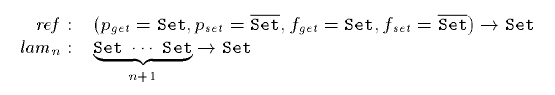
\includegraphics[scale=0.3]{andersen_constructor_signatures.png}
    \end{figure}
  \item Having $\alpha$ renamed the program variables, we can be sure
    each is unique, and use the inference rules in \boldit{And+Common}.
  \end{itemize}

  \framebreak

  \begin{figure}
    \centering
    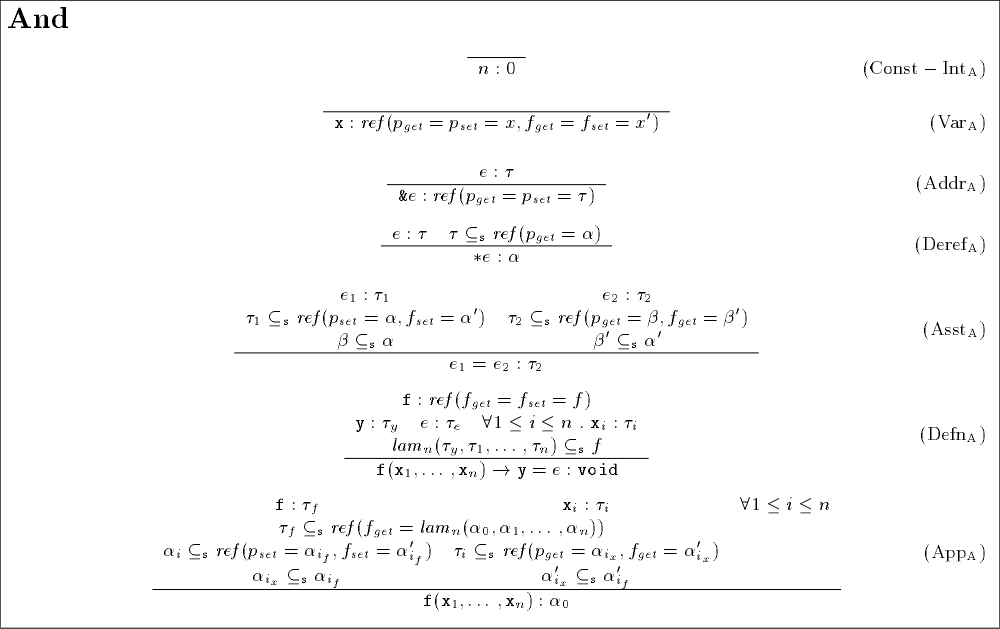
\includegraphics[scale=0.3]{andersen_inference_rules.png}
  \end{figure}

  \framebreak

  \begin{figure}
    \centering
    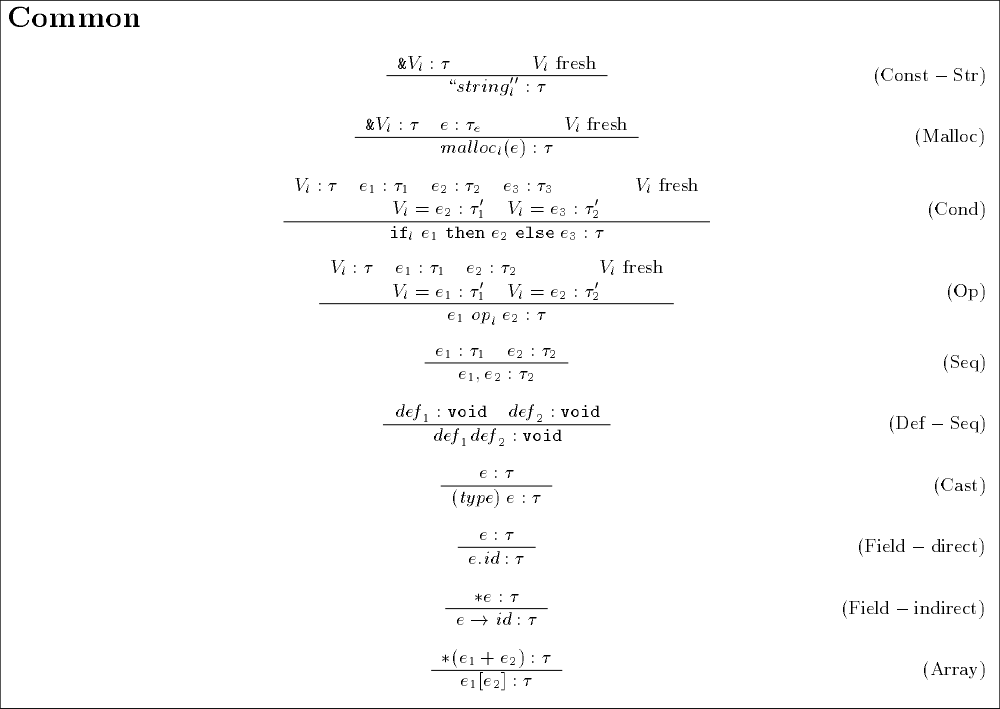
\includegraphics[scale=0.3]{common_inference_rules.png}
  \end{figure}

  \framebreak

  \begin{itemize}
  \item Let $\vdash_A$ mean "provable in \boldit{And+Common}".
  \item Then, Andersen's points-to relation $P_A: L \rightarrow 2^L$
    is given by $ y \in P_A(x) $ if 
    $$ CS \vdash_A ref(p_{get}=p_{set}=y, f_{get}=f_{set}=y') \subseteq_s x $$
  \end{itemize}

\end{frame}

\begin{frame}[allowframebreaks]
  \frametitle{Steensgard-style analysis}

  \begin{itemize}
  \item In this system, types follow this grammar.
    \begin{figure}
      \centering
      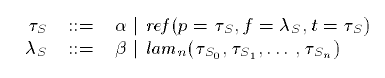
\includegraphics[scale=0.3]{steensgard_type_grammar.png}
    \end{figure}
  \item The constructors $ref$ and $lam_n$ have these signatures.
    \begin{figure}
      \centering
      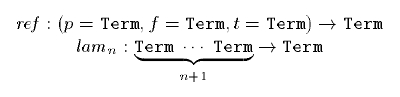
\includegraphics[scale=0.3]{steensgard_constructor_signatures.png}
    \end{figure}
  \item Steensgard's system uses unification where Andersen's had
    inclusion, thus: 
    \begin{itemize}
    \item the old $p_{get}$(covariant) and $p_{set}$(contravariant)
      merge into $p$(invariant).
    \item the old $f_{get}$(covariant) and $f_{set}$(contravariant)
      merge into $f$(invariant).
    \item the field $t$ is added to store a tag; this refers to the
      equivalence class the reference belongs to.
    \end{itemize}
  \item Having $\alpha$ renamed the program variables, we can be sure
    each is unique, and use the inference rules in \boldit{Ste+Common}.
  \end{itemize}

  \framebreak

  \begin{figure}
    \centering
    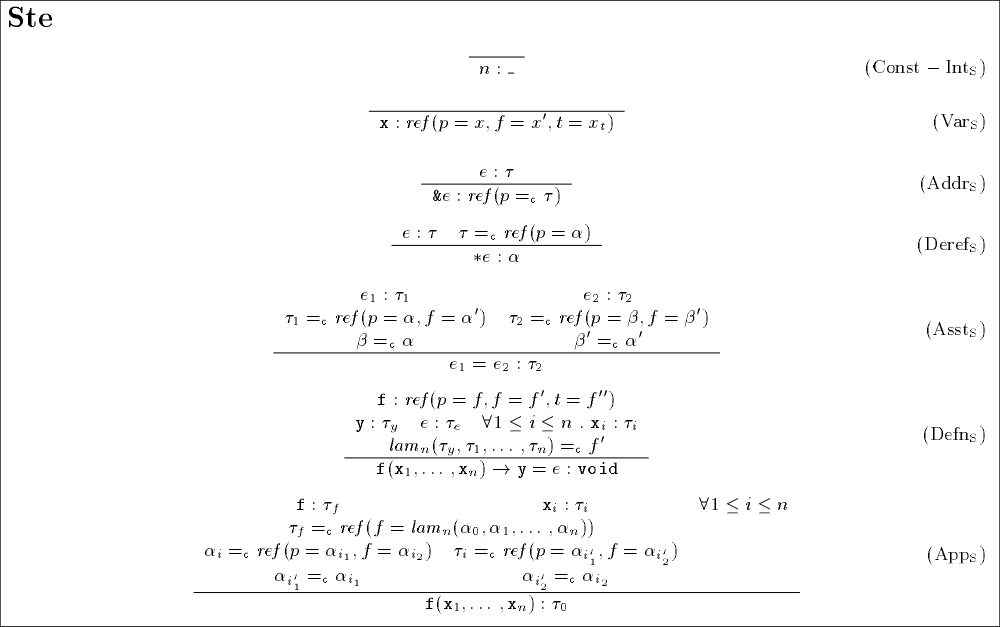
\includegraphics[scale=0.3]{steensgard_inference_rules.png}
  \end{figure}

  \framebreak

  \begin{itemize}
  \item In this analysis, $x =_c y$ (conditional unification) iff
    $$ \exists c. \vdash c(\dotso) \eg_t x \Rightarrow x_t y $$
    Intuitively, conditionally unified terms are unified only when one
    of them is unified with a constructed type.
  \item Let $\vdash_S$ mean "provable in \boldit{Ste+Common}".
  \item Then, Steensgard's points-to relation $P_S: L \rightarrow 2^L$
    is given by $ y \in P_S(x) $ if 
    $$ CS \vdash_S ref(p=y, f=y', t = y_t) =_t x $$
  \item In this system, the equivalence class $[x]$ containing a memory
    location $x$ is given by $[x] = {y: CS \vdash_S x_t = y_t }$
  \end{itemize}

\end{frame}

\begin{frame}[allowframebreaks]
  \frametitle{Exploiting the correspondence between Andersen's and
    Steengard's analyses}

  \begin{itemize}
  \item These two analyses are similar enough that we can build a
    common system, \boldit{Comb} that can implement either, only
    changing the constructor signatures.
  \item This is the type grammar.
    \begin{figure}
      \centering
      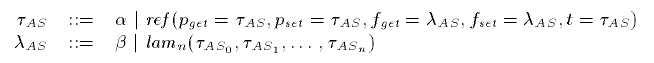
\includegraphics[scale=0.3]{combination_type_grammar.png}
    \end{figure}
  \item For the Andersen-style analysis, we use these constructor
    signatures. The $t$ field is ignored.
    \begin{figure}
      \centering
      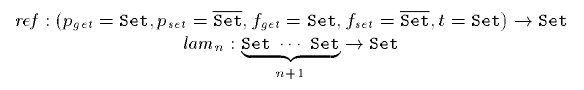
\includegraphics[scale=0.3]{combination_andersen_constructor_signatures.png}
    \end{figure}
  \item For the Steensgard-style analysis, we use these constructor
    signatures. $p_{get} = p_{set}$ and $f_{get} = f_{set}$ are required.
    \begin{figure}
      \centering
      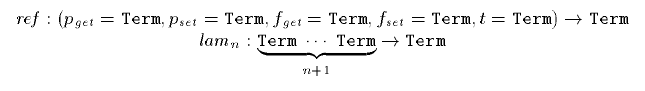
\includegraphics[scale=0.3]{combination_steensgard_constructor_signatures.png}
    \end{figure}

  \end{itemize}

  \framebreak

  \begin{figure}
    \centering
    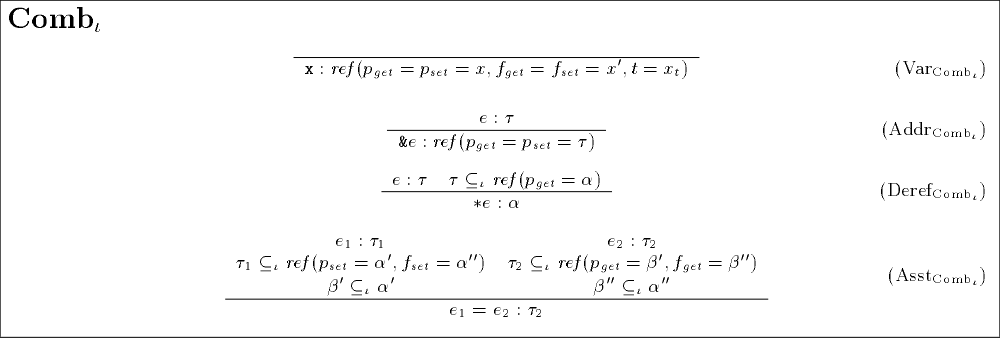
\includegraphics[scale=0.3]{combination_inference_rules.png}
  \end{figure}

  %% \framebreak

  \begin{itemize}
  \item The rules for this system are similar to those in
    \boldit{And}; The rules for function definition and application
    remain the same.
  \item For Andersen-style analysis, use subset constraints
    ($\subseteq_{\iota} = \subseteq_s$) and constraint system $CS_s$.
  \item For Steensgard-style analysis, use conditional equality
    constraints ($\subseteq_{\iota} = \subseteq_c$) and constraint
    system $CS_c$ .
  \item The parameterised points-to relation $Q_{\iota} : L
    \Rightarrow 2^L $ is given by $y \in Q_{\iota}(x)$ if:
    $$ CS_{\iota} \vdash ref(p_{get}=p_{set}=y, f_{get}=f_{set}=y',
    t=y_t) \subseteq_{\iota} x $$
  \item This lemma shows the equivalence between the points-to sets
    generated by \boldit{And+Common} and $\boldit{Comb_{s} + Common}$,
    and also those generated by \boldit{Ste+Common} and
    $\boldit{Comb_{c}+Common}$.
    \begin{figure}
      \centering
      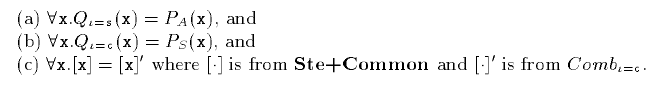
\includegraphics[scale=0.3]{lemma_7_2.png}
    \end{figure}
  \item Next lemma: Andersen-style subset inclusion
    is a sufficient condition for Steensgard-style conditional
    unification. More formally, if the system $CS_s$ is translated to
    the system $CS_c$ (i. e. each $\tau_1 \subseteq_s \tau_2$
    translated to $\tau_1 =_c \tau_2$), then
    $$ CS_s \vdash \tau_1' \subseteq_s \tau_2' \Rightarrow CS_c \vdash \tau_1' =_c \tau_2' $$
  \item Using these two lemmas, it's simple to show that $$ y \in
    P_A(x) \Rightarrow y \in P_s(x) $$
  \item Pretty cool, right?

  \end{itemize}

\end{frame}

\begin{frame}[allowframebreaks]
  \frametitle{Soundness}

  \begin{itemize}
  \item For a soundness result, we'll have to construct operational
    semantics for a fragment of C - best to keep it simple.
    $$ e ::= x | *e | \& e | e_1 = e_2 | e1,e2 $$
  \item Let's construct a mapping $\theta$ from dynamic memory
    locations $Loc$ to syntactic locations $SyntacticLoc$.
    \begin{figure}
      \centering
      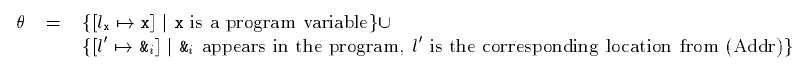
\includegraphics[scale=0.3]{theta.png}
    \end{figure}
  \item Program transformation: every time the address of a variable
    appears in an expression, add a new program variable $\&_i$ to
    store the result and substitute $\&_i$ in the result. The type
    inference rule is fairly obvious.
    \begin{figure}
      \centering
      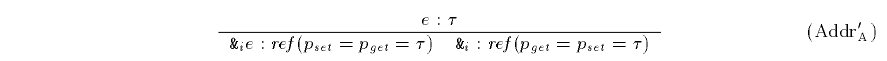
\includegraphics[scale=0.3]{theta_inference_rule.png}
    \end{figure}
  \end{itemize}

  \framebreak

  \begin{figure}
    \centering
    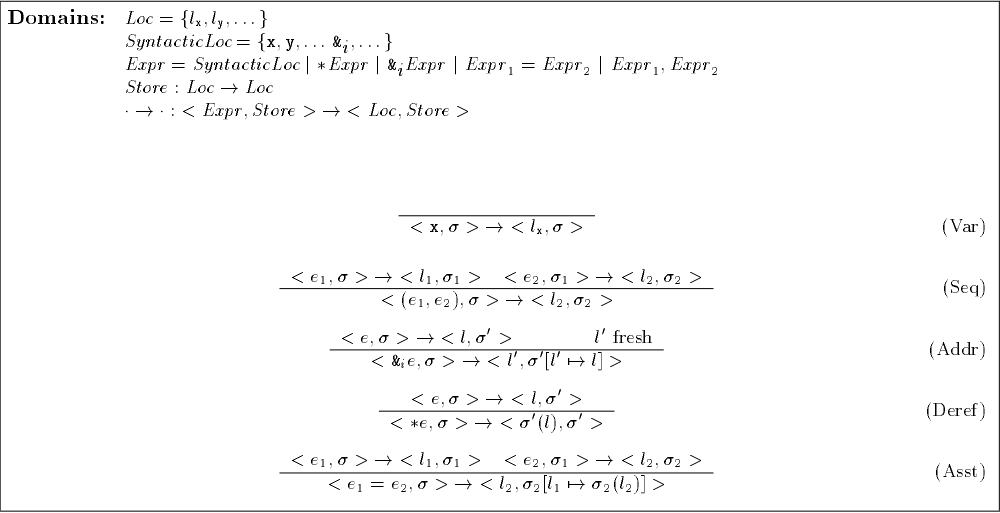
\includegraphics[scale=0.3]{operational_semantics.png}
  \end{figure}

  \framebreak

  \begin{itemize}
  \item For each syntactic location $x$, let $\phi(x)$ be the type
    $\tau$ such that $\vdash_A x: ref(p_{get} = p_{set} =
    \tau)$. If $x$ is a program variable, then $\phi(x) = x$.
  \item From this, we get a result showing something like an upper and
    lower bound for Andersen-style analysis.
    \begin{figure}
      \centering
      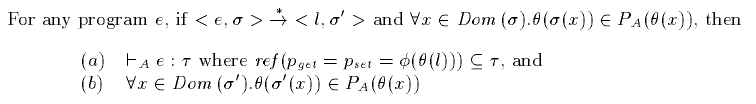
\includegraphics[scale=0.3]{theorem_7_6.png}
    \end{figure}
  \item From this, we have a final result showing the soundness of
    both Andersen's and Steensgard's analyses.
    \begin{figure}
      \centering
      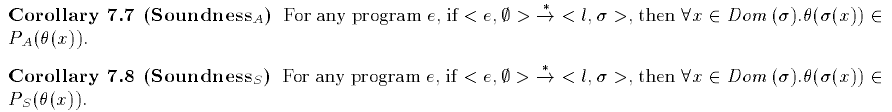
\includegraphics[scale=0.3]{corollary_7_7_and_7_8.png}
    \end{figure}

  \end{itemize}
\end{frame}

\begin{frame}[allowframebreaks]
\frametitle{Implementation and results}

  \begin{figure}
    \centering
    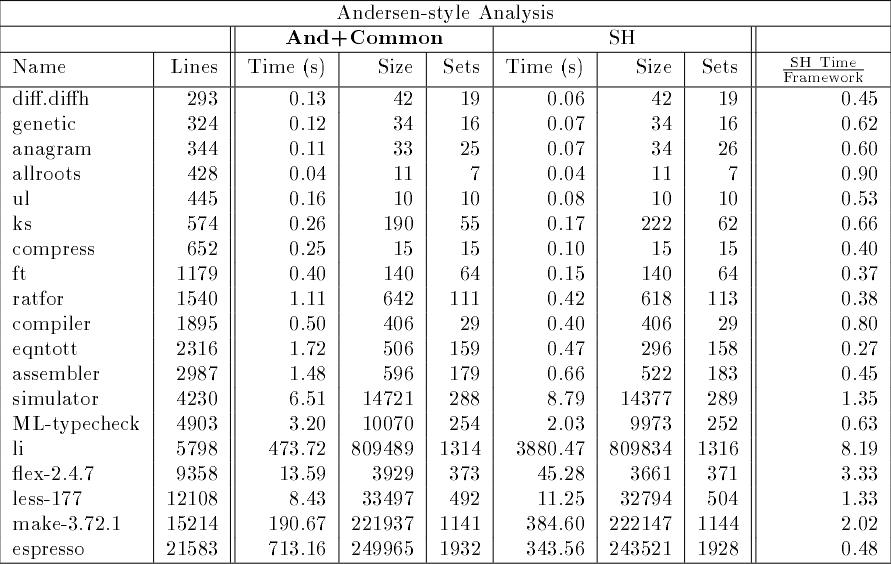
\includegraphics[scale=0.3]{andersen_comparison.png}
  \end{figure}

  \begin{figure}
    \centering
    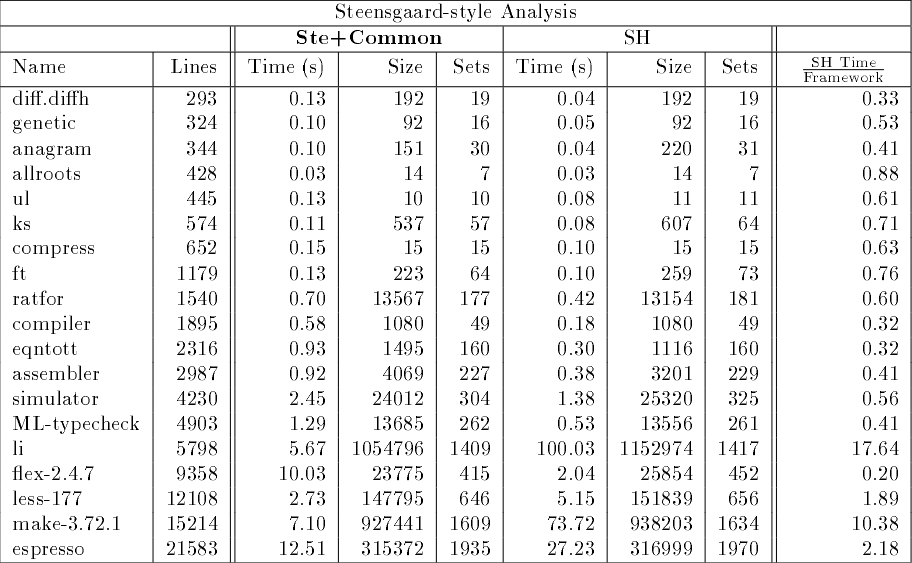
\includegraphics[scale=0.3]{steensgard_comparison.png}
  \end{figure}
\end{frame}

\begin{frame}[allowframebreaks]
  \frametitle{References}
  \bibliographystyle{plain}
  \bibliography{citeseerx,Aiken99,CharatonikP94}
\end{frame}

\end{document}
